\section{Triển khai và đánh giá hệ thống}
\subsection{Triển khai hệ thống}
\subsubsection{Triển khai Web Service}
Hệ thống chúng tôi được triển khai như sau:
\begin{enumerate}[-]
    \item Deploy Server: Sử dụng Google Cloud để triển khai Web serivce với cấu hình 
    \item Cơ sở dữ liệu PosgreSQL: Sử dụng Aiven.io để triển khai cơ sở dữ liệu PosgreSQL, với cấu hình 1GB RAM / 1 Core CPU / 5Gb Storage.
    \item Cơ sở dữ liệu Neo4j: Sử dụng  neo4j Aura để triển khai cơ sở dữ liệu đồ thị với cấu hình 1GB RAM / 1 Core CPU / 5Gb Storage.
    \item Lưu trữ: Sử dụng service S3 của AWS để triển khai cho việc lưu trữ hình ảnh.
\end{enumerate}
Các bước triển khai hệ thống:

\begin{enumerate}[1.]
    \item \textbf{Chuẩn bị sẵn các dịch vụ sử dụng}: Ta cần tạo 1 máy ảo từ Google Cloud chạy hệ điều hành Linux và 1 database PosgreSQl từ Aiven và 1 cở sở dữ liệu Neo4j từ Aura.
    \item \textbf{Thiết lập khoá trên máy ảo}: Để có thể cấp quyền Pull code trên máy ảo, ta cần tạo khoá công khai và thêm vào tài khoản Git.
    \item \textbf{Tải và cập nhật các thư viện:} Chúng ta cần cập nhập thư viện có trong máy ảo và cài nginx, node, pm2 bằng các câu lệnh sau:\cite{deploy}
     \begin{enumerate}[-]
        \item sudo apt-get update
        \item sudo apt-get install nginx
        \item sudo systemctl start nginx
        \item sudo apt-get install nodejs
        \item sudo npm install pm2 -g
     \end{enumerate}
    \item \textbf{Thiết lập mã nguồn}: Sau khi Pull code về tạo ra file .env và bỏ tất cả các biến môi trường vào file này. Sau đó thực hiện lệnh build. Sau đó ta khởi chạy dự án với pm2 và kiếm tra trạng thái
    \begin{enumerate}[-]
        \item pm2 start dist/index.js
        \item pm2 status
    \end{enumerate}
    \item \textbf{Thiết lập nginx:} Thiết lập nginx cho các yêu cầu tới Nodejs. Ta mở tệp cấu hình nginx và cấu hình lại, proxy\_pass ta cần điền port mà ứng dụng chạy.
    \begin{enumerate}[-]
        \item sudo nano /etc/nginx/sites-available/default
        \item  \begin{figure}[H]
        \centering
        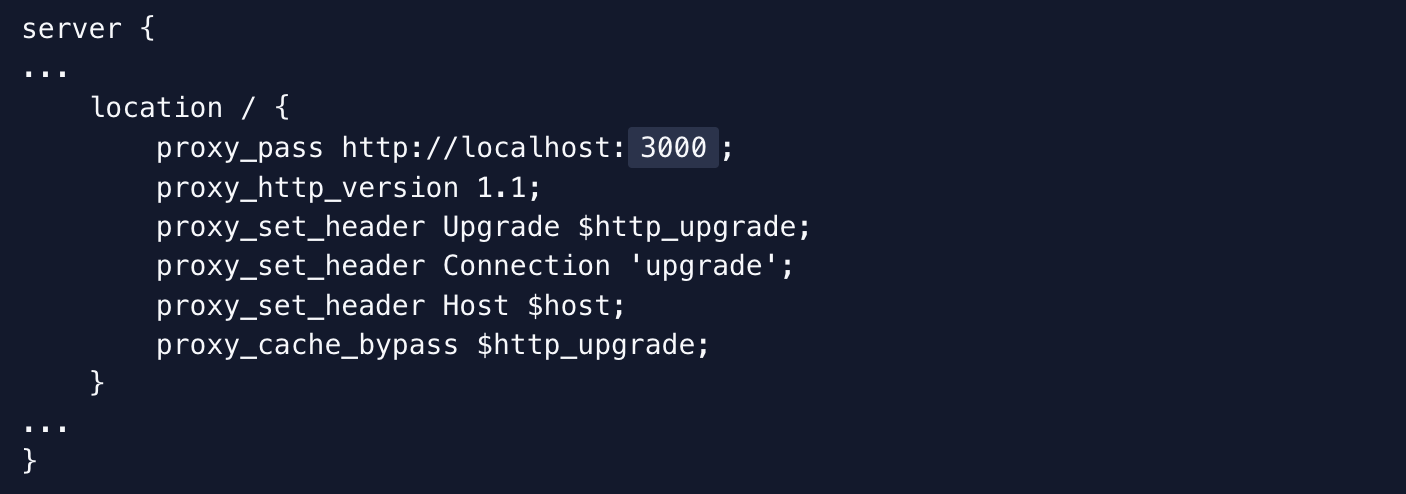
\includegraphics[width=10cm]{Images/Trienkhai/BE/nginxConfig.png}
        \newline
        \caption{Cấu hình nginx}
    \end{figure}
    \end{enumerate}
    \item \textbf{Kết quả: } Kiểm thử và khởi chạy lại nginx và ứng dụng đã được deploy thành công
    \begin{enumerate}[-]
        \item sudo systemctl restart nginx
    \end{enumerate}
\end{enumerate}
\subsubsection{Triển khai Website Admin trên Cloudflare}
Nhóm sử dụng dịch vụ của CloudFlare để triển khai trang web cho admin quản lý và mua tên miền từ id.tenten.vn. Các bước được thực hiện như sau:
\begin{enumerate}[1.]
    \item \textbf{Đăng ký tài khoản CloudFlare:} Đầu tiên chúng ta cần vào trang web của CloudFlare và tạo tài khoản nếu chưa có. Sau đó thực hiện đăng nhập.
    
    \item \textbf{Khởi tạo dự án:} Ở trang Dashboard, ở thanh sidebar chọn "Workers \& Pages" rồi chọn "Overview". Nội dung trang hiện ra ta chọn tiếp nút "Create Application"
    \begin{figure}[H]
        \centering
        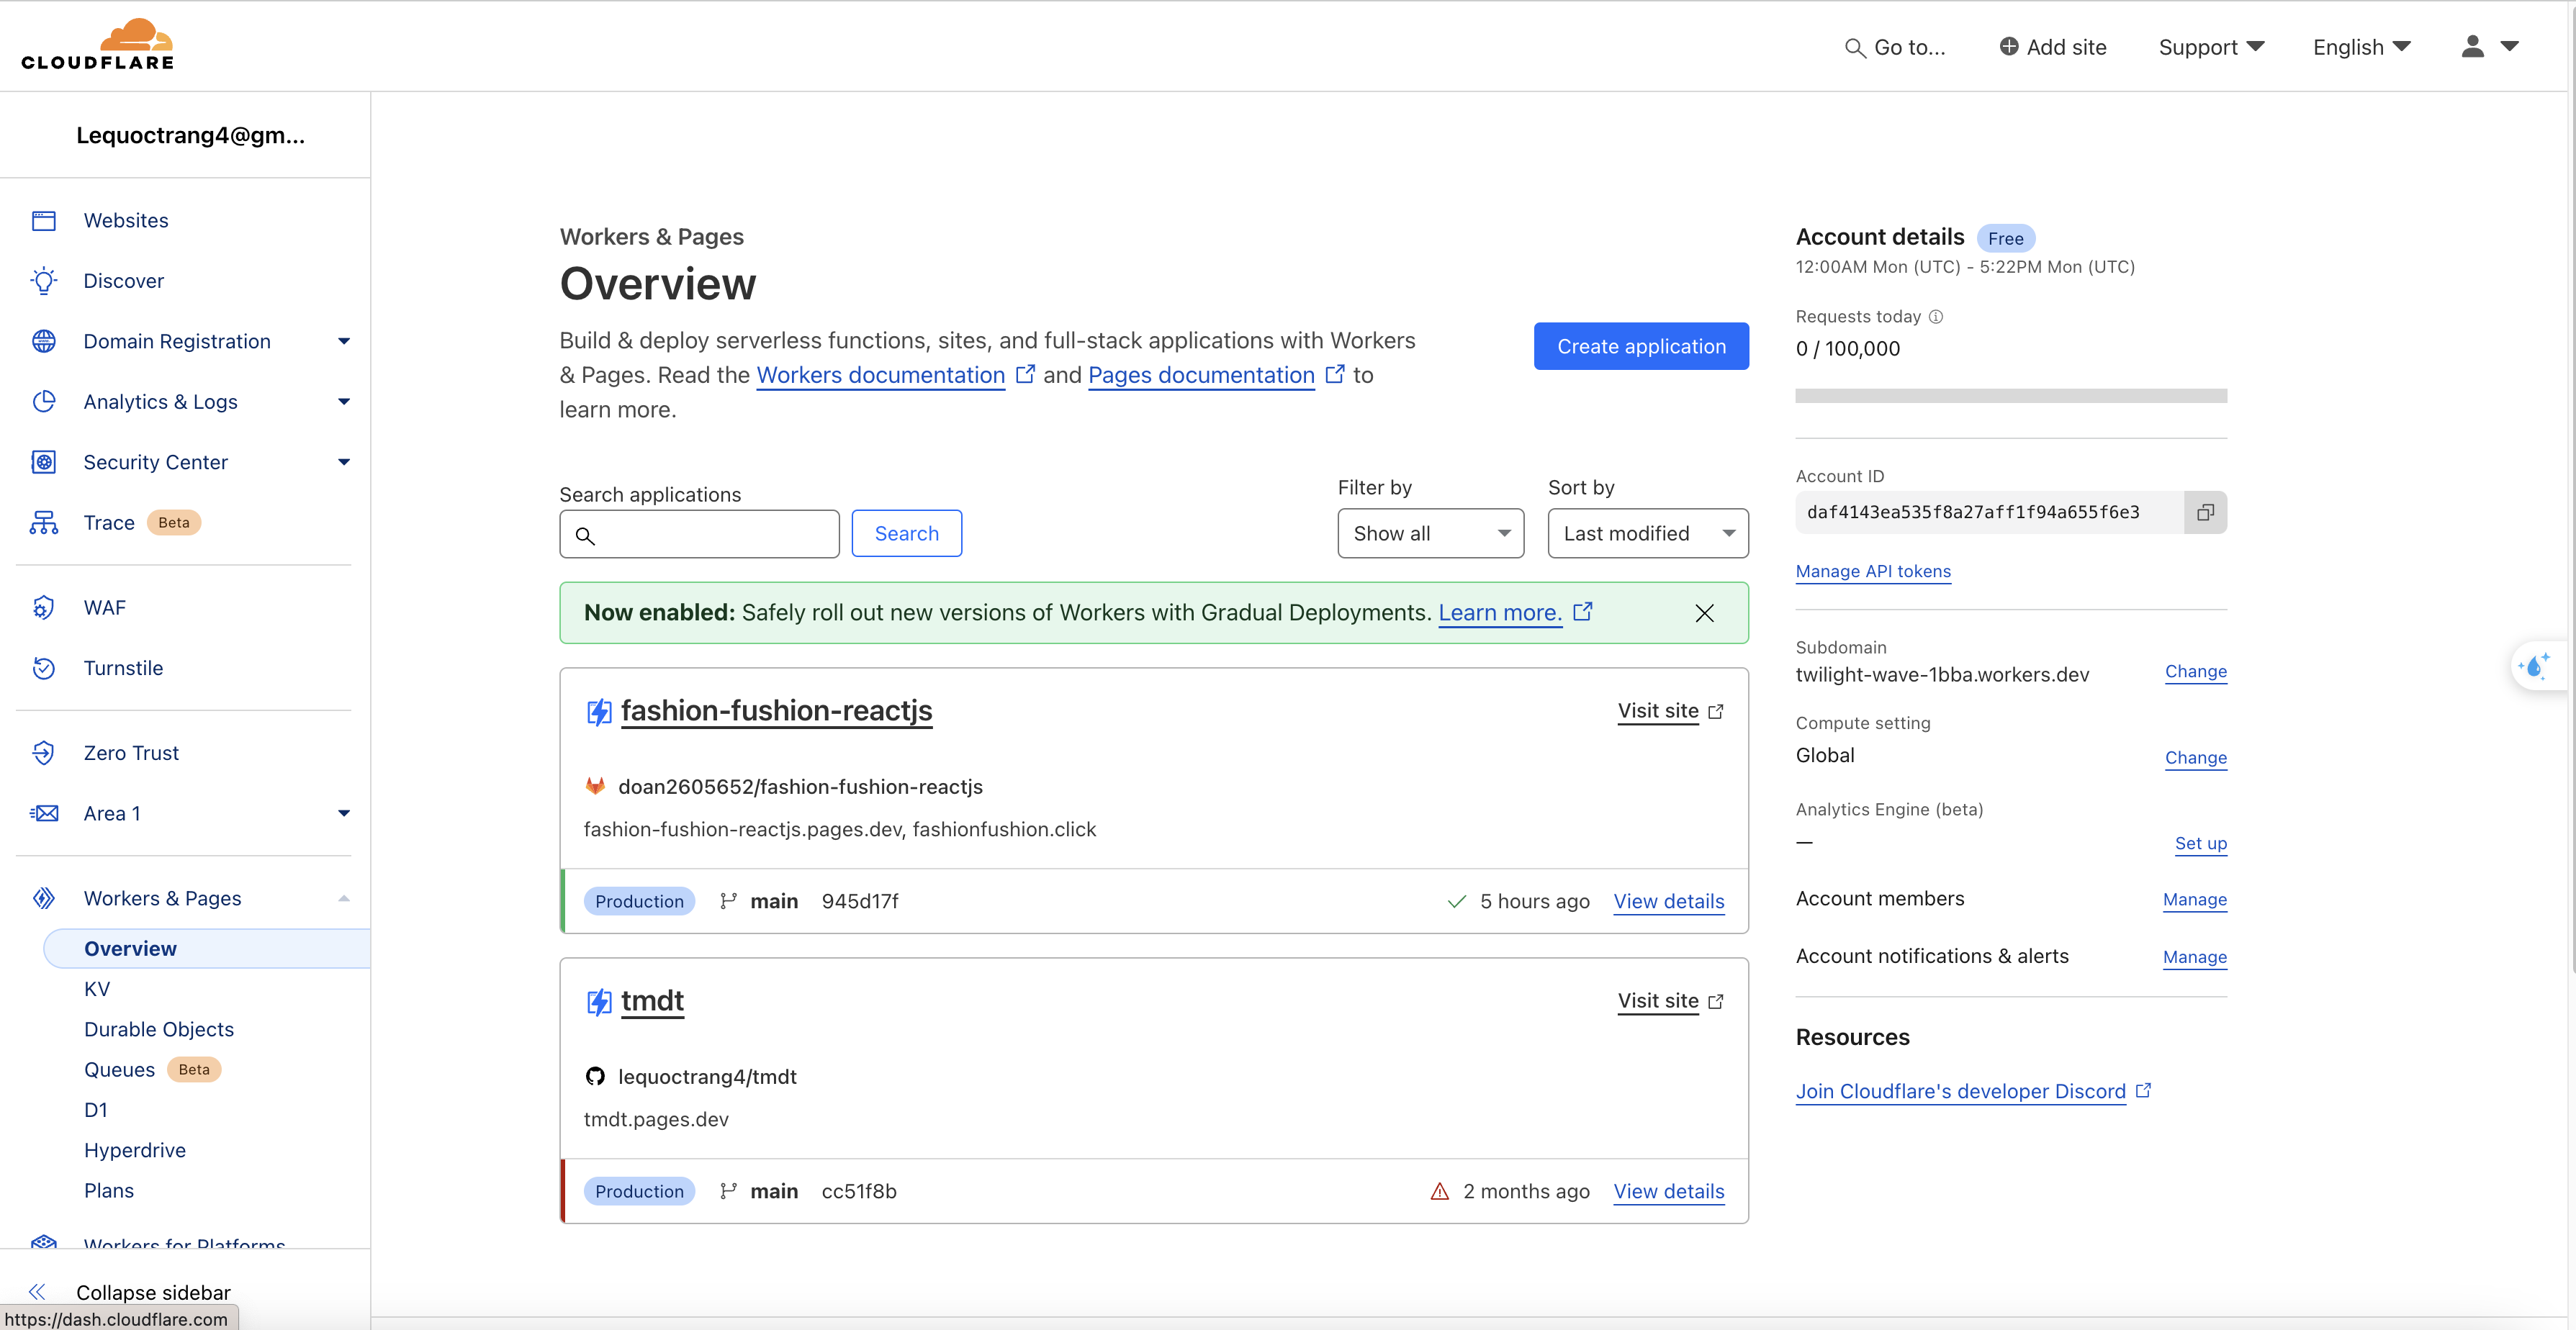
\includegraphics[width=16cm]{Images/Trienkhai/Web/step2.png}
        \newline
        \caption{Khởi tạo dự án trên CloudFlare}
    \end{figure}
    \item \textbf{Liên kết đến Git}: Sau đó chọn Mục "Page" và chọn "Connect To Git". Sau đó ta chọn dự án cần triển khai và chọn "Begin setup"
    \item  \textbf{Cấu hình dự án:} Sau khi tạo dự án, ta cần cấu hình dự án của mình. Đầu tiên cần chọn nhánh deploy là nhánh main. Sau đó ở phần "Framework preset" ta chọn "Create React App" thì CloudFlare sẽ tự xác định thư mục build và câu lệnh run build. Nếu chúng ta có sử dụng những câu lệnh build khác hay là chỉnh "Build output directory" thì cần phải sửa lại cho đúng. Tiếp theo là "Root Directory" và thiết lập các biến môi trường ở phần "Environment variables". Cuối cùng bấm "Save \& Deploy".
     \begin{figure}[H]
        \centering
        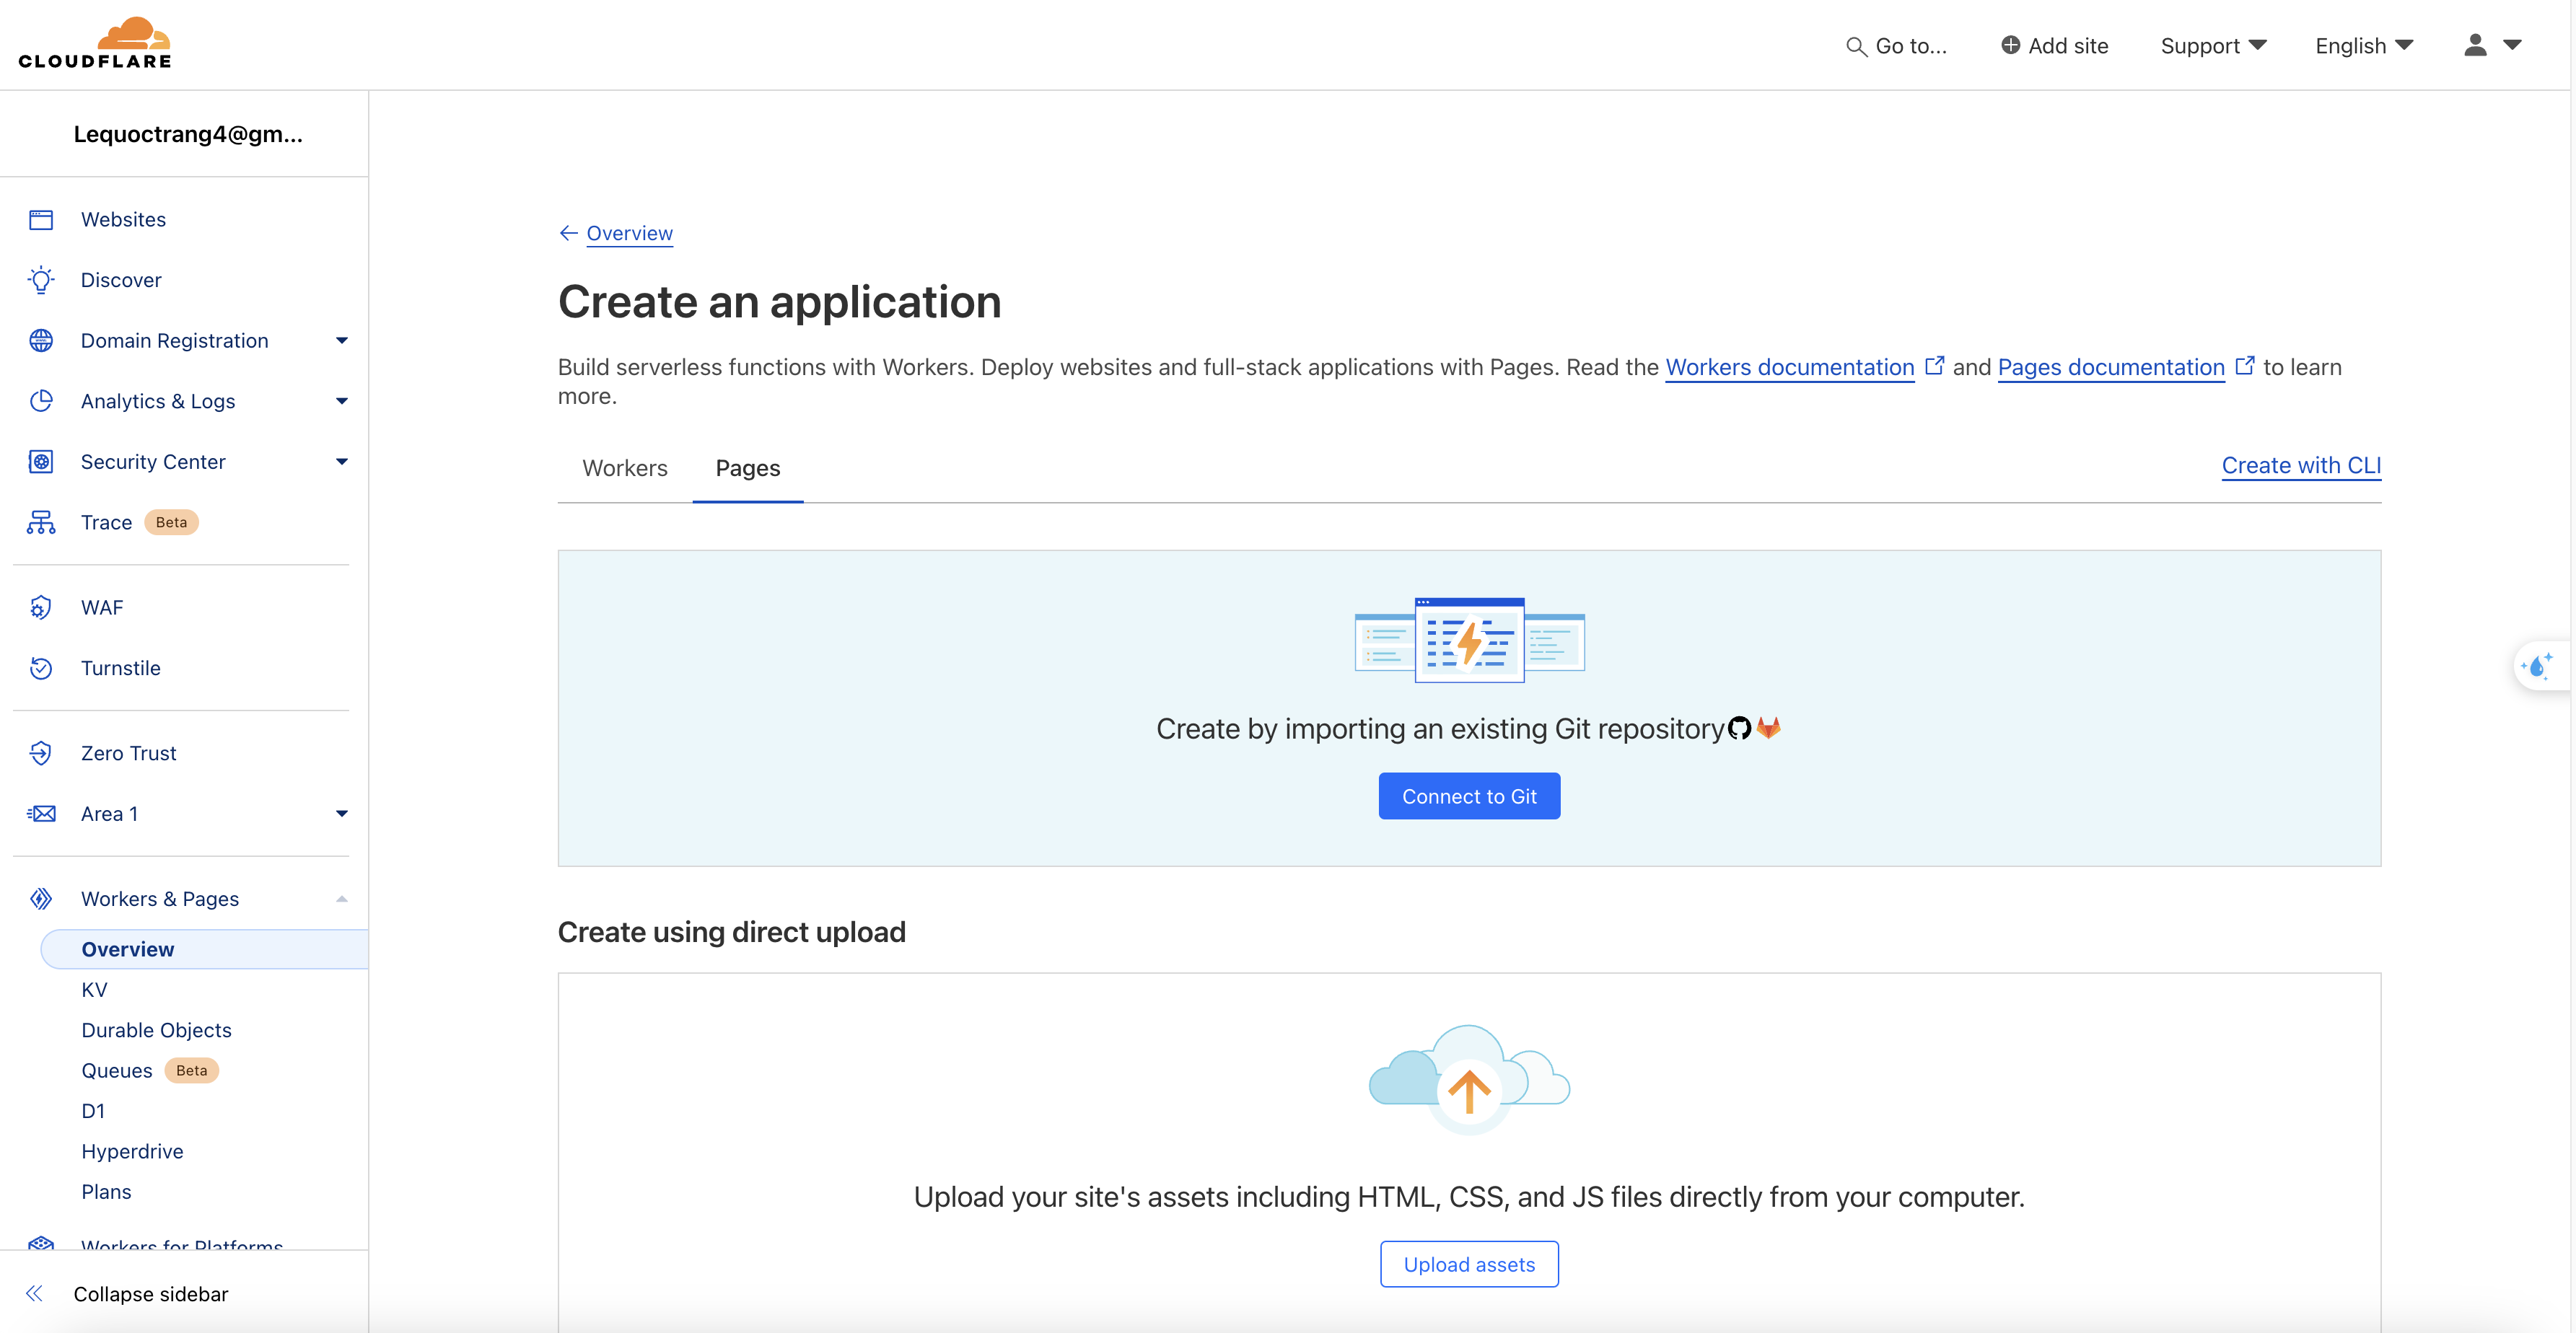
\includegraphics[width=16cm]{Images/Trienkhai/Web/step4.png}
        \newline
        \caption{Thiết lập các biến môi trường và tiến hành Deploy}
    \end{figure}
    
    \item \textbf{Xem kết quả:}  Sau khi triển khai thành công, CloudFlare sẽ cung cấp URL có thể sử dụng để xem ứng dụng đã triển khai.
\end{enumerate}
\subsubsection{Triển khai tên miền}
Sau khi mua được tên miền thì chúng tôi sẽ gắn tên miền đến địa chỉ IP của hệ thống và trang web. Ở đây chúng tôi sử dụng CloudFlare để thực hiện quản lý tên miền. Các bước được thực hiện như sau:

\begin{enumerate}[1.]
    \item \textbf{Xác thực tên miền: } Sau khi đăng nhập vào CloudFlare, ở mục thanh bên trái, chọn "Websites" rồi chọn "Add a site", sau đó điền tên miền đã chuẩn bị và thực hiện xác thực. Để thực hiện việc xác thực tên miền, ta cần thêm đường dẫn của Cloudflare cung cấp để thêm vào name server của tên miền.
    \item  \textbf{Thiết lập DNS: } Ở trang quản lý tên miền, ta chọn "DNS" -> "Record" ở thanh điều hướng bên trái. Sau đó bấm "Add record". Đối với Server thì ta cần chọn type là "A" vì cần nhập địa chỉ IPv4 còn đối với trang web thì ta chọn "CNAME"
\end{enumerate}
\begin{figure}[H]
    \centering
    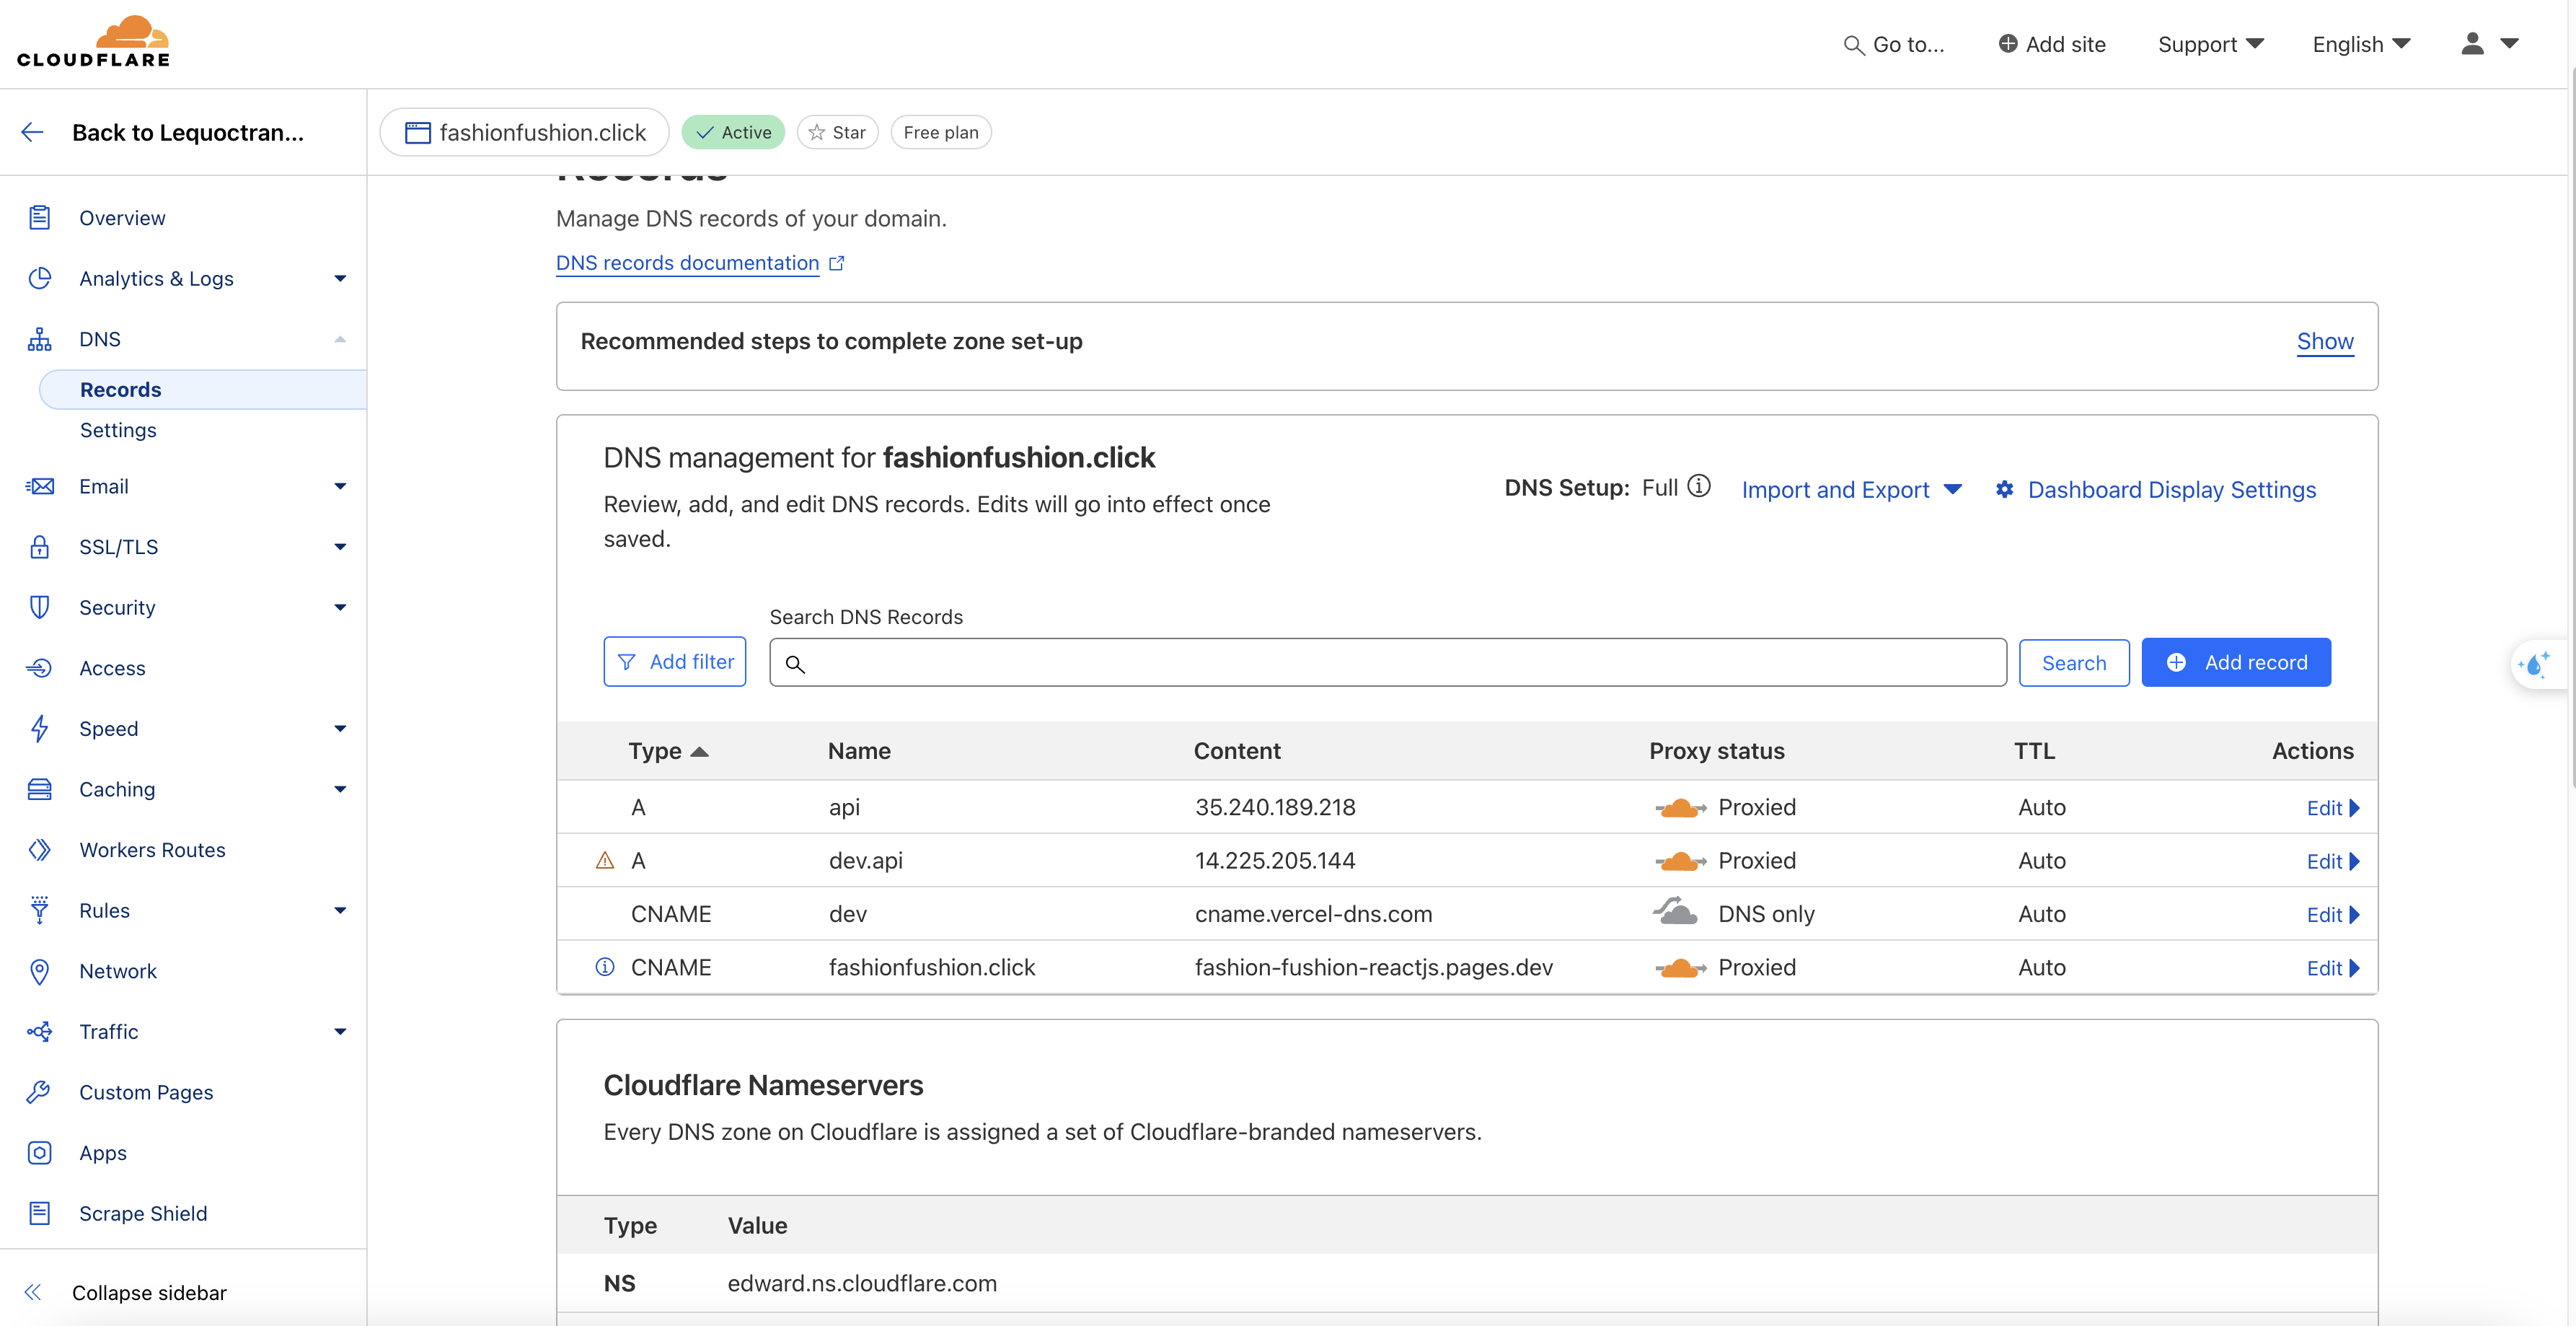
\includegraphics[width=15cm]{Images/Trienkhai/dns.png}
    \newline
    \caption{Thiết lập DNS cho tên miền}
\end{figure}
Sau khi thực hiện thiết lập tên miền thì đường dẫn Web service api và trang web như sau:
\begin{itemize}
    \item \textbf{Môi trường develop}: môi trường dành cho nhà phát triển
    \begin{itemize}
        \item Backend Api: https://dev.api.fashionfushion.click
        \item Website Admin: https://dev.fashionfushion.click
    \end{itemize}
    \item \textbf{Môi trường production}: môi trường dành cho thương mại
    \begin{itemize}
        \item Backend Api: https://api.fashionfushion.click
        \item Website Admin: https://fashionfushion.click
    \end{itemize}
\end{itemize}

\subsection{Đánh giá hệ thống}
\subsubsection{Đánh giá hiệu suất hệ thống bằng Google PageSpeed Insights}
Hiệu suất tải trang web là một yếu tố quan trọng đối với trải nghiệm người dùng của các ứng dụng web. Nhận thức được điều này, chúng tôi đã tiến hành đánh giá bằng cách sử dụng công cụ PageSpeed Insights của Google Chrome. PageSpeed Insights không chỉ giúp đánh giá hiệu suất mà còn đưa ra các khuyến nghị để cải thiện tốc độ tải của ứng dụng web. Chúng tôi sử dụng PageSpeed Insights để đánh giá ứng dụng web đã được triển khai trên Cloudflare.\\
 \begin{figure}[H]
        \centering
        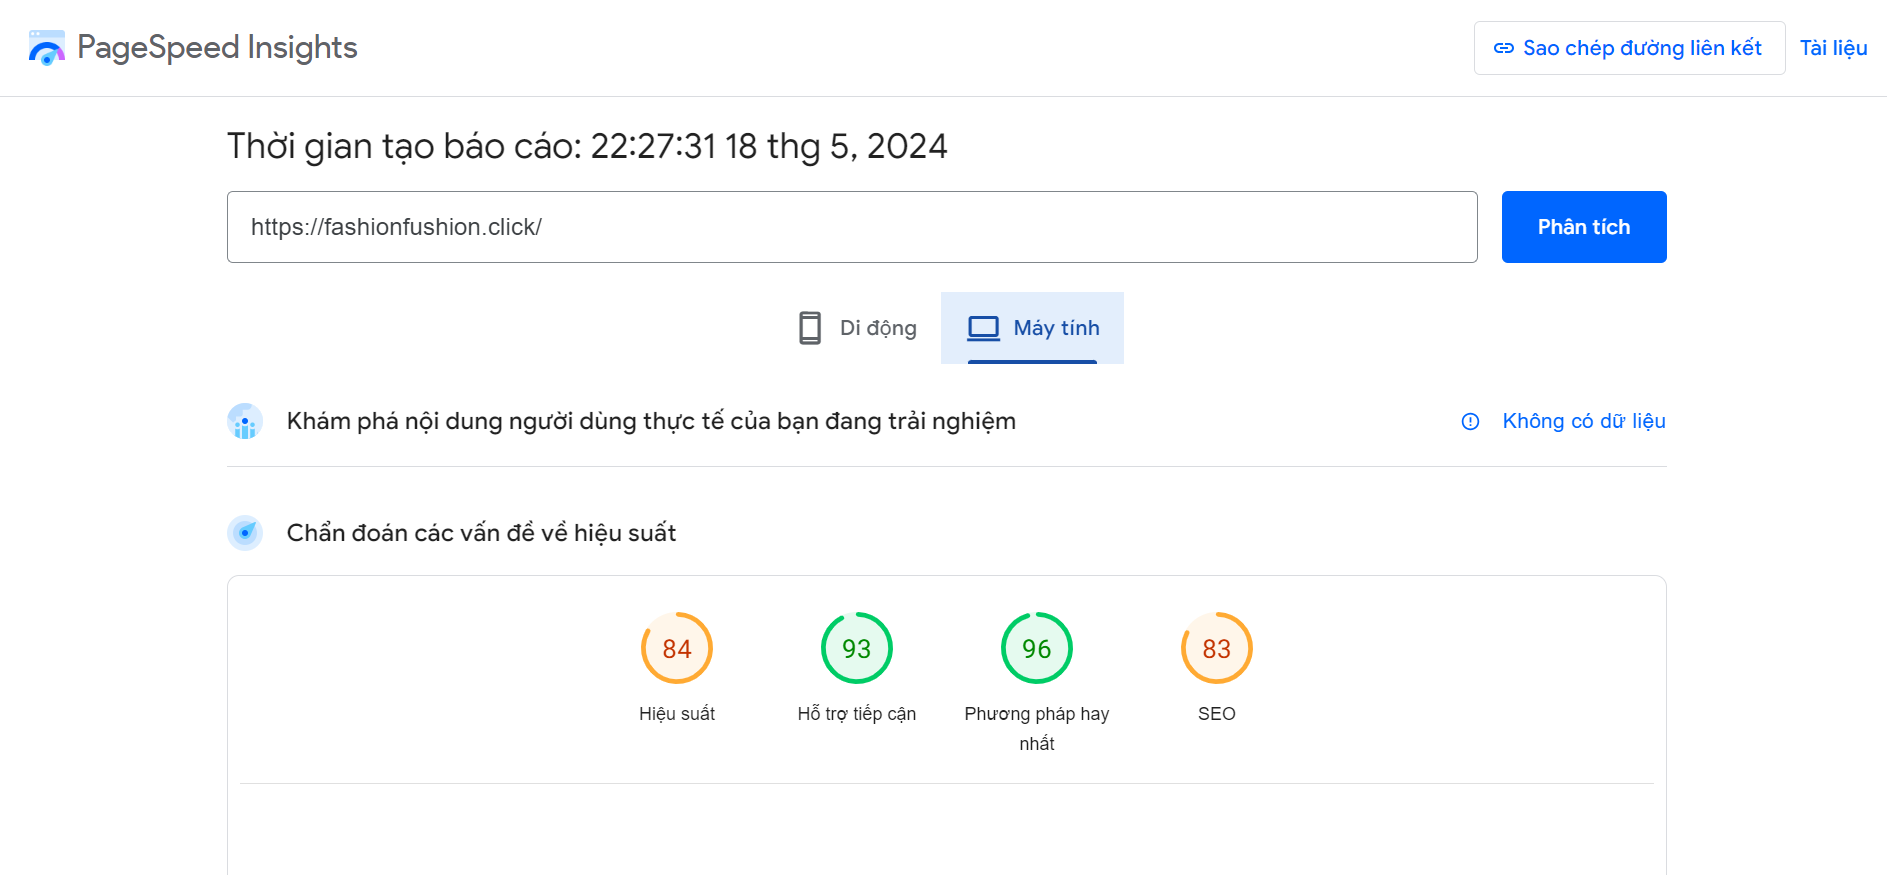
\includegraphics[width=16cm]{Images/hieusuat.png}
        \newline
        \caption{Điểm đánh giá PageSpeed Insights lần đầu tiên}
    \end{figure}